\subsection{Depth Camera Testing}
\label{subsec:depthcameratesting}

\begin{figure} [ht]
  \centering
  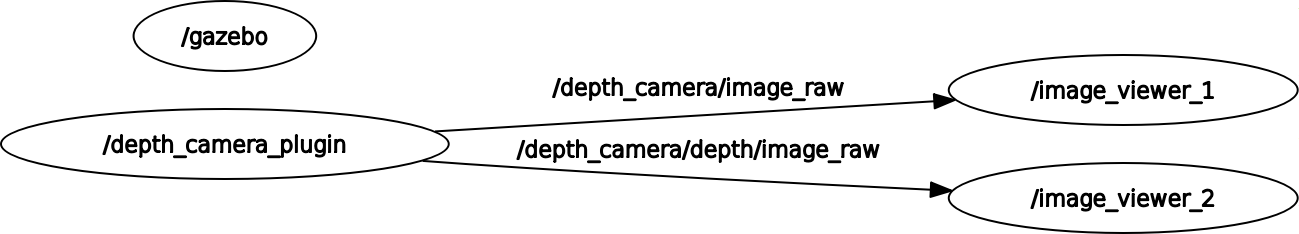
\includegraphics[width=0.45\textwidth]{figures/rosgraph/depth-camera-sim.png}
  \IfLanguageName{english}{
    \caption{Node scheme of the depth camera testing in the simulation.}
  }{
    \caption{Skema \emph{node} dari pengujian \emph{depth camera} di simulasi.}
  }
  \label{fig:rosgraphdepthcamerareal}
\end{figure}

\begin{figure} [ht]
  \centering
  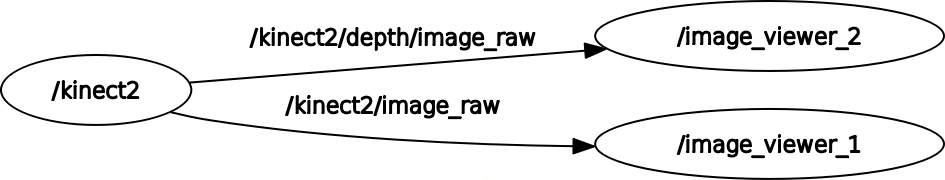
\includegraphics[width=0.45\textwidth]{figures/rosgraph/depth-camera-real.png}
  \IfLanguageName{english}{
    \caption{Node scheme of the depth camera testing on the real robot.}
  }{
    \caption{Skema \emph{node} dari pengujian \emph{depth camera} pada robot fisik.}
  }
  \label{fig:rosgraphdepthcamerareal}
\end{figure}


Depth camera testing is done to test the ability of depth camera in the simulation to simulate the depth camera device,
  while at the same time to test the hardware abstraction in the ROS 2.
This test is done by running two \lstinline{image_viewer} nodes that each of which will receive color images and depth images.
As shown in figure \ref{fig:rosgraphdepthcamerasim},
  in the simulation,
  each \lstinline{image_viewer} nodes will receive color image data using the \lstinline{/depth_camera/image_raw} topic and depth image data using the \lstinline{/depth_camera/depth/image_raw} topic.
As for the testing in the real world,
  as shown in figure \ref{fig:rosgraphdepthcamerareal},
  the role of the \lstinline{depth_camera_plugin} node will be replaced by \lstinline{v4l2_camera} node that will send data which came from the Kinect V2 device on the real robot.

\begin{figure} [ht]
  \centering
  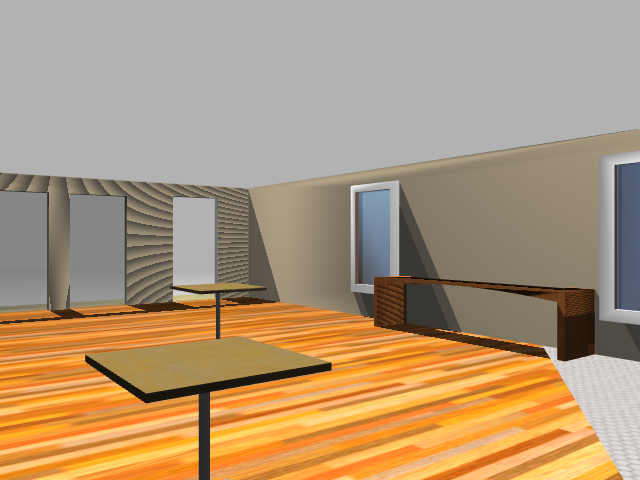
\includegraphics[width=0.225\textwidth]{figures/depth-camera/sim-rgb.png}
  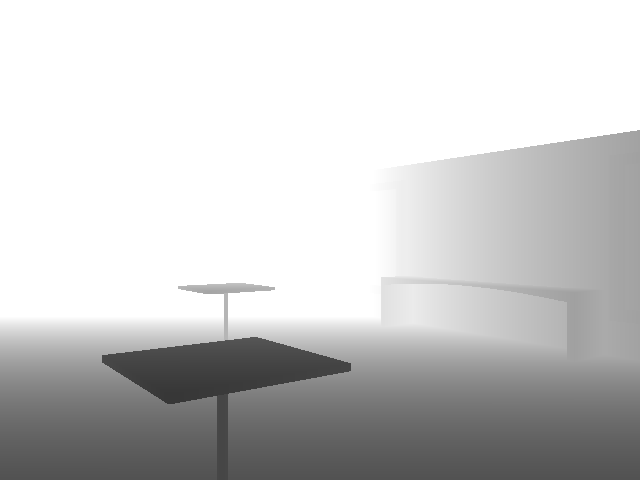
\includegraphics[width=0.225\textwidth]{figures/depth-camera/sim-depth.png}
  \IfLanguageName{english}{
    \caption{Comparison of the depth camera capture results in the simulation.}
  }{
    \caption{Perbandingan hasil tangkapan \emph{depth camera} di simulasi.}
  }
  \label{fig:depthcameraresultsim}
\end{figure}


The result,
  as shown in figure \ref{fig:depthcameraresultsim},
  \lstinline{image_viewer} node will display the data received from the simulation in which the left image (\ref{fig:depthcameraresultsimrgb}) shows a colored image,
  while the right image (\ref{fig:depthcameraresultsimdepth}) shows a depth image with black and white display.
In the depth image,
  the brighter a point in the image indicates a position that is far from the center point of the camera.

\begin{figure} [ht]
  \centering
  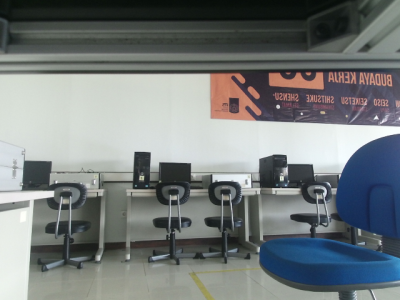
\includegraphics[width=0.225\textwidth]{figures/depth-camera/real-rgb.png}
  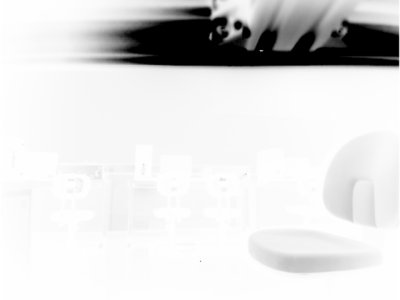
\includegraphics[width=0.225\textwidth]{figures/depth-camera/real-depth.png}
  \IfLanguageName{english}{
    \caption{Comparison of the depth camera capture results on the real robot.}
  }{
    \caption{Perbandingan hasil tangkapan \emph{depth camera} pada robot fisik.}
  }
  \label{fig:rosgraphdepthcamerareal}
\end{figure}


Meanwhile,
  on the real robot the obtained results are also relatively the same.
As shown in figure \ref{fig:depthcameraresultreal},
  the left image (\ref{fig:depthcameraresultrealrgb}) indicates a colored image while the right image (\ref{fig:depthcameraresultrealdepth}) indicates a depth image.
However,
  in those images,
  the depth image has a brighter result,
  this happens because the range of the Kinect V2 is shorter (4.5 meter) than the range that was set on the depth camera in the simulation.
